\documentclass[a4paper,12pt]{article}
\usepackage[utf8]{inputenc}
\usepackage{graphicx}
\usepackage[english]{babel}
\usepackage{geometry}
\usepackage{setspace}
\usepackage{minted}
\usepackage{booktabs}

\geometry{margin=1in}
\onehalfspacing

\begin{document}

\begin{titlepage}
    \begin{center}
        
\includegraphics[width=0.4\textwidth]{images/uni_logo.jpg} \\[1cm] % adjust the logo here
        {\Large \textbf{Genetic Data Analysis of Rheumatoid arthritis and Clouston's disease}} \\[1cm] % Title
        \textit{Module: M1 Méthodologie de traitement de données NGS} \\[3cm] % Subtitle

        \vfill % to push the authors to the bottom of the page

        \textbf{Authors} \\[0.5cm]
        \textsc{Ngoc VU, Denys BURYI}


    \end{center}
\end{titlepage}

\newpage


\section*{Introduction}

We have carried out linkage analyses (lod-score or affected sib-pairs) 
and association analyses (case-control or familial) for a monogenic disease, then for a multifactorial disease:
\begin{enumerate}
    \item Study of a monogenic disease: Clouston's disease
    \begin{enumerate}
        \item Genetic linkage analysis (lodscore)
        \item Familial association analysis
    \end{enumerate}
    \item Study of a multifactorial disease: rheumatoid arthritis
    \begin{enumerate}
        \item Genetic linkage analysis (affected sib-pairs)
        \item Genome-Wide case-control association analysis
    \end{enumerate}
\end{enumerate}

 
The data and programs were provided by our professor VALÉRIE CHAUDRU.

\section{Monogenic disease: Clouston's disease}

Clouston syndrome is mainly characterized by abnormal nails (thickened, slow-growing, brittle) 
and alopecia (hair loss). \textit{Palmoplantar hyperkeratosis} (commonly known as horniness) is 
also sometimes observed. 
This is a rare disease, with a prevalence ranging from 1 to 9 in 100,000. It is autosomal dominant. 
Penetrance of the disease is complete, but its expression is variable, even in patients from the same family.
Our aim in this part of the analysis was to:

\begin{itemize}
    \item Perform linkage analysis using the lodscore method to locate the Clouston disease gene 
    using genetic markers located on chromosome 13.
    \item Interpret data from a \texttt{.vcf} file containing genetic variants identified in a 
    case-control sample and perform association analysis for a candidate variant.
    \item Search for the causal genetic variant using familial association analysis.
\end{itemize}

\subsection{Genetic linkage analysis - lodscore method}

We have analyzed the data contained in the \texttt{fam.txt} file using \texttt{paramlink} package in R. 
First we performed some initial data exploration using \texttt{linkdat()} and \texttt{summary()} functions:

    
    \begin{minted}[frame=lines, linenos]{r}
        fam = read.table('fam.txt')
        x = linkdat(fam)
        summary(x)
        \end{minted}


\newpage
We found that the file contains data of a large family of 47 individuals, comprising 22 affected and
 25 unaffected members. These individuals are organized into 10 nuclear subfamilies and 
have been genotyped for 13 genetic markers on chromosome 13. For 11 individuals in the dataset no 
parent data was available (further reffered to as "founders"). Figure \ref{fig:pedigree} shows 
the pedigree plot of the family.

\begin{figure}[ht!] % ht! means here at the top, despite placing rules 
    \centering
    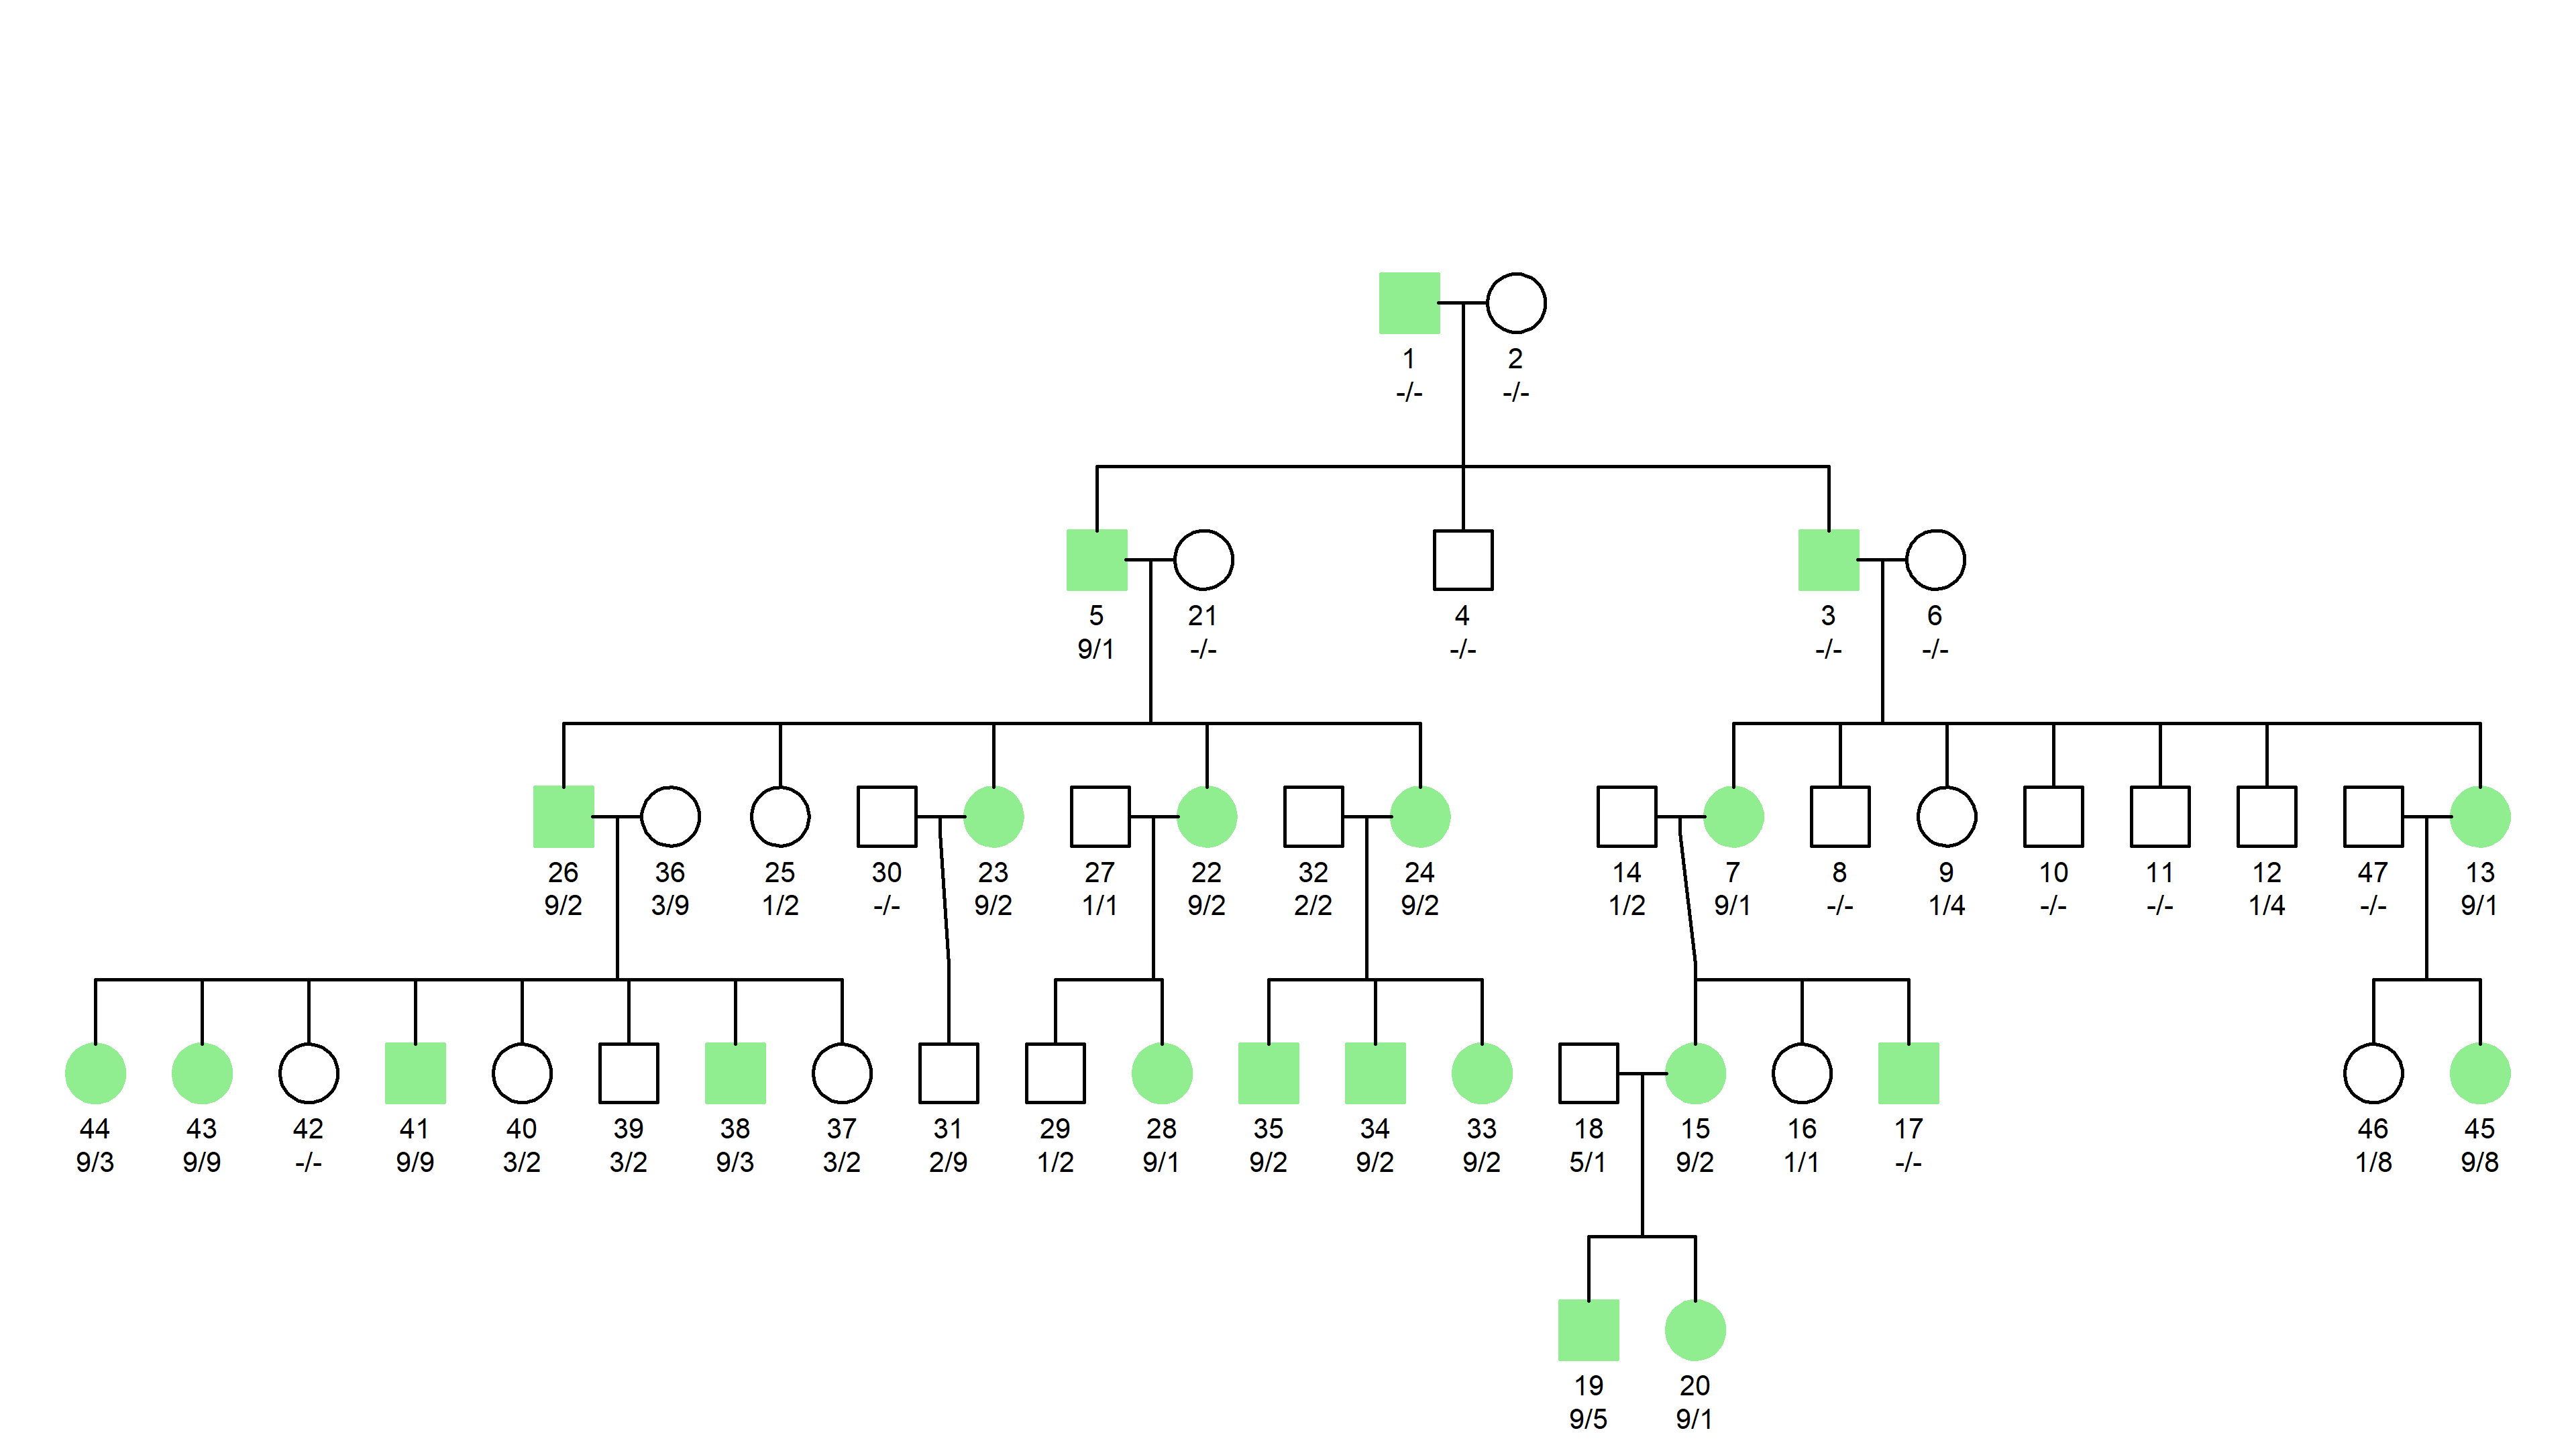
\includegraphics[width=\textwidth]{images/pedigree_plot.png}
    \caption{Pedigree plot of the family along with their affection status and genotypes with 
    regards to marker 1.
    Affected - light green, Unaffected - white. Sex: square/circle - M/F. Genotype: alleles of the marker 1.}
    \label{fig:pedigree} % this allows to reference the figure with \ref{fig:pedigree}

    
\end{figure}

In addition to helping summarize the data, the \texttt{linkdat()} function also transforms the original data
and outputs a \texttt{linkdat} object that can be used to perform linkage analysis. \texttt{linkdat} object 
is a list containing among others, the following important components:
\begin{itemize}
    \item \texttt{pedigree} - data.frame with 5 columns (ID, FID, MID, SEX, AFF) describing the pedigree in linkage format.
    \item \texttt{orig.ids} - vector of original IDs of the individuals in the pedigree.
    \item \texttt{subnucs} - list of vectors of IDs of individuals in each nuclear family.
    \item \texttt{markerdata} - a list of \texttt{marker} objects describing information about the genetic markers.
\item \texttt{model} - a list of parameters for the linkage analysis.
\end{itemize}



\subsection{Mode of inheritance: Autosomal Dominant}

First, we have analyzed our data assuming an autosomal dominant mode of inheritance. Using the \texttt{setmodel()} function,
we have set the parameters to:
\begin{itemize}
    \item phenocopies = $10^{-5}$
    \item complete penetrance
    \item disease allele frequency = $10^{-5}$
\end{itemize}

We then performed the linkage analysis using the \texttt{lod()} function for a range of $\theta$ from 0 to 0.5 with a step of 0.05. 
We have saved the results in the \texttt{result\_dom} data frame for further analysis (see code below).

\begin{minted}[frame=lines, linenos]{r}
    xdom = setModel(x, model=1, penetrances = c(0.00001, 1, 1), dfreq = 0.00001)
    result_dom = lod(xdom, theta=c(0, 0.05, 0.1, 0.15, 0.2, 0.25, 0.3, 0.4, 0.5)) 
    result__dom_df = as.data.frame(result_dom)
\end{minted}

\begin{figure}[hb!] % b for bottom 
    \centering
    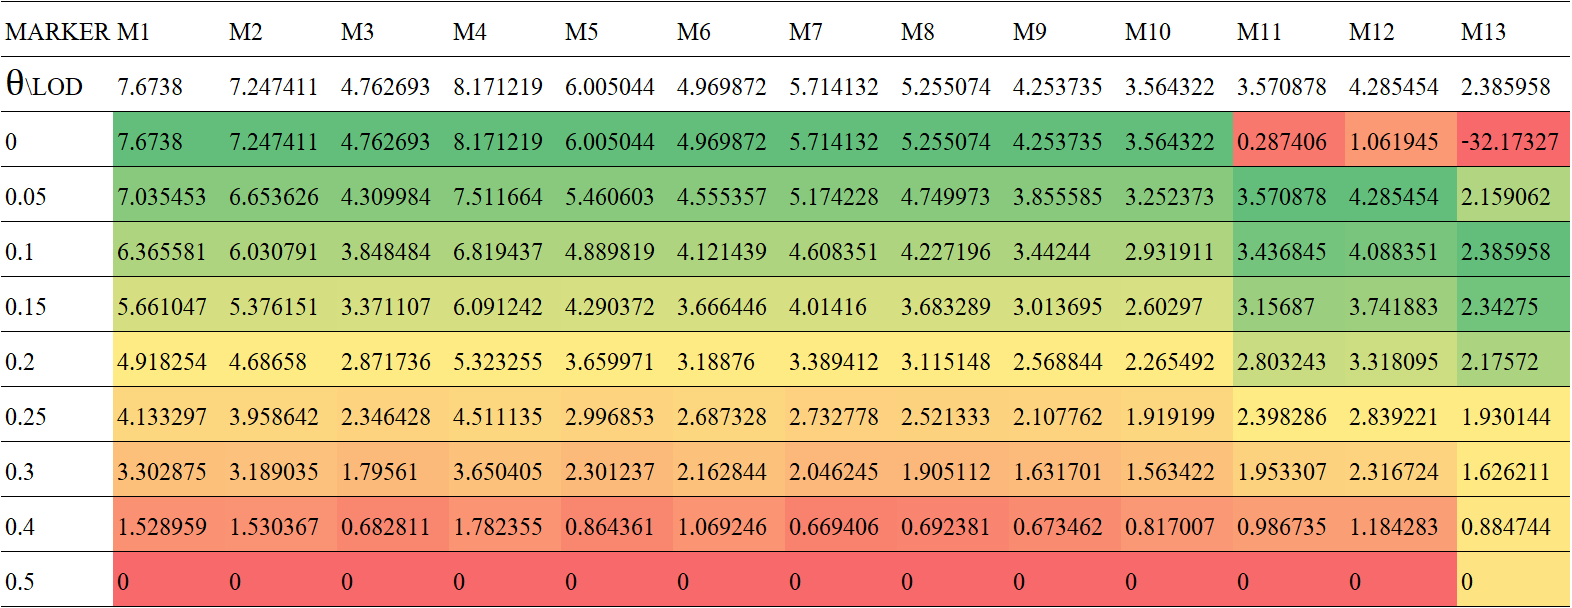
\includegraphics[width=\textwidth]{images/xdom_lod_analysis.png}
    \caption{LOD score analysis results for autosomal dominant mode of inheritance. Each column shows 
    Lod-score for a given marker, for a given $\theta$ value. Top row shows maximum Lod-score for each marker. 
    Conditional coloring: green to red - higest to lowest Lod-score.}   
    \label{fig:xdom_lodscore} 
    
\end{figure}

Based on the results shown in the figure \ref{fig:xdom_lodscore}, we can conclude that 
the disease gene is at extrimely close proximity to markers 1-10, at 5 cM distance 
from markers 11 and 12, and at 15 cM distance from marker 13. To confirm these findings, 
we have performed the same analysis for $\theta$ values from 0 to 0.05 with a step of 0.01 (see figure \ref{fig:xdom_lodscore_granular}).

\begin{figure}[t] % t for top 
    \centering
    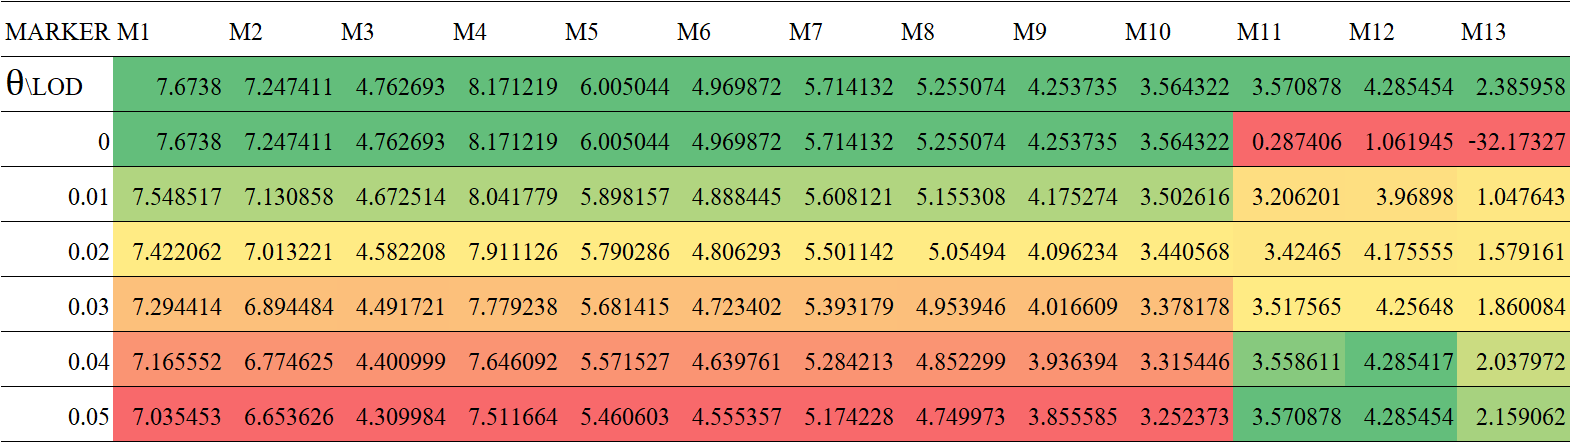
\includegraphics[width=\textwidth]{images/xdom_lod_analysis_more_granular.png}
    \caption{LOD score analysis results for autosomal dominant mode of inheritance for more 
    granular $\theta$ values. Each column shows Lod-score for a given marker, for a given 
    $\theta$ value. Top row shows maximum Lod-score for each marker. Conditional coloring: 
    green to red - higest to lowest Lod-score.}   
    \label{fig:xdom_lodscore_granular} 
    
\end{figure}



\newpage
    \section{Multifactorial disease: Rheumatoid Arthritis}

\end{document}